\input{configuration}

\title{Lecture 31 --- Live Kernel Patching}

\author{Jeff Zarnett \\ \small \texttt{jzarnett@uwaterloo.ca}}
\institute{Department of Electrical and Computer Engineering \\
  University of Waterloo}
\date{\today}


\begin{document}

\begin{frame}
  \titlepage
\end{frame}


\begin{frame}
\frametitle{Can't Stop Won't Stop}

\begin{center}
	
\includegraphics[width=0.6\textwidth]{images/batcountry.jpg}
\end{center}

When people are counting on a system -- particularly life and safety-critical ones -- it might be difficult to schedule a maintenance window for it.

\end{frame}


\begin{frame}
\frametitle{Uptime is Everything}

Let's say that we cannot, or at least do not want to, have a system restart for the purposes of updating the kernel. 

It is perhaps not the right choice to disrupt a long-running task, but also not great to leave security vulnerabilities unaddressed until a maintenance window.

We need a third option: change the kernel without a reboot. Or in other words, we are trying to maximize availability.

\end{frame}


\begin{frame}
\frametitle{Staged Rollout}

Many modern software projects allow for some sort of staged or transitional rollout.

That does not work for the kernel! 

Not on the same machine anyway -- we could do this kind of warm handover if we're replacing a machine with another. 

\end{frame}


\begin{frame}
\frametitle{We Have A Method}

As we learned earlier, kernels have the ability to load and unload new modules. 

So if what we need is to unload \& reload a kernel module, that's not too difficult. 

Let's say the vulnerability we want to fix is that there's a bug in the device driver for an attached sensor. 

Great, we can probably pause (quickly!) things that use it, unload the kernel module, load the new one, and resume execution.

\end{frame}


\begin{frame}
\frametitle{Bug in the Kernel?}

But if the bug is in the kernel itself? 

That requires changing the kernel's main functionality. And doing it live. 

Can we load some code into the kernel and have it replace existing things?

\end{frame}


\begin{frame}
\frametitle{Self Surgery}

In practice, this is a little bit like the kernel doing a surgery on itself.

\begin{center}
	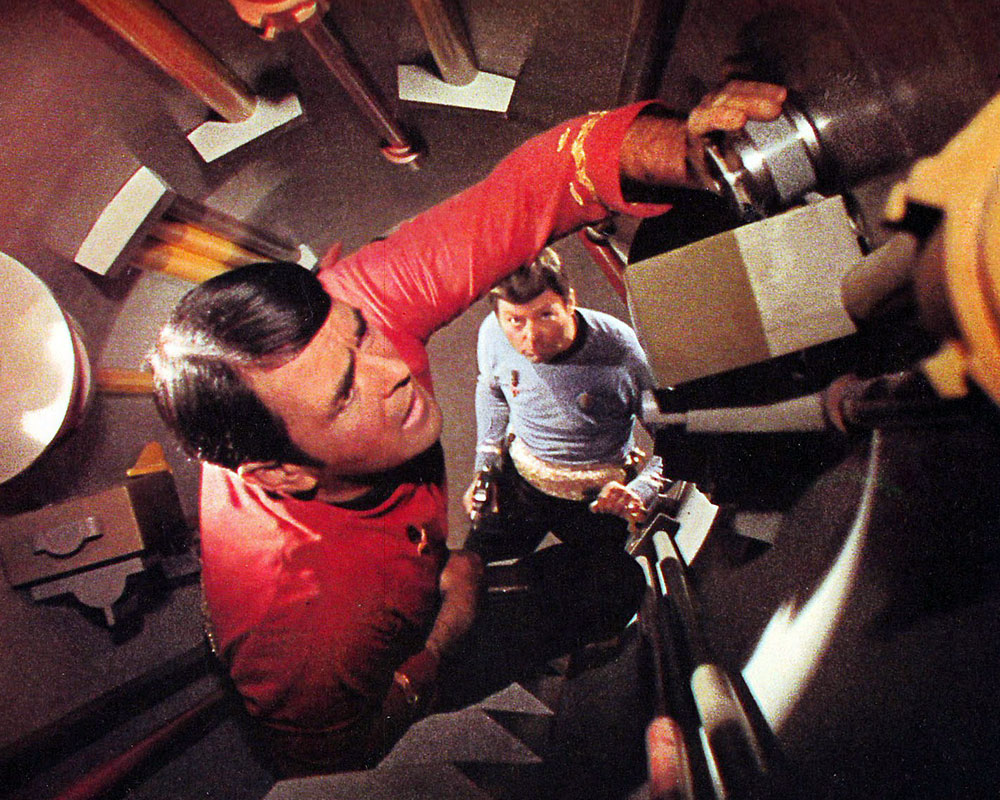
\includegraphics[width=0.5\textwidth]{images/jeffries.jpg}
\end{center}

\end{frame}


\begin{frame}
\frametitle{Basic Plan}

Step one: validate that we can make this change at all.

Step two: prepare the patch.

Step three: make sure it is safe to make the swap.

Step four: execute the replacement.

\end{frame}


\begin{frame}
\frametitle{How Complex?}

Kernel docs say: many fixes do not change the semantics.

\begin{itemize}
	\item Add a \texttt{NULL} pointer or a boundary check.
	\item Fix a race by adding a missing memory barrier.
	\item Add some locking around a critical section.
\end{itemize}

Most of these changes are self contained and the function presents itself the same way to the rest of the system.

\end{frame}

\begin{frame}
\frametitle{We Can Do Hard Things}

The patching mechanism can be used to do a larger change than just one of these ``typical'' cases. 

The consequences of getting this wrong are potentially severe:\\
\quad Crash (kernel panic), silent corruption, etc.

Or we could introduce security vulnerabilities instead of fix them.

\begin{center}
	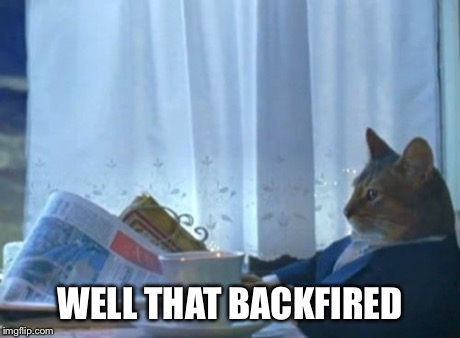
\includegraphics[width=0.4\textwidth]{images/backfire.jpg}
\end{center}

\end{frame}


\begin{frame}
\frametitle{\texttt{kpatch} and \texttt{kGraft}}

There were two competing approaches: \texttt{kpatch} and \texttt{kGraft}.\\
\quad The final version took some of each.

Both mechanisms aim to do a replacement of a function within the running kernel; the new code is loaded as a module (akin to a driver) into that kernel. 

Then, calls to the old function are intercepted and redirected to the new.

\end{frame}


\begin{frame}
\frametitle{Finding the Place}

There's a little nuance about how to find the place to patch in the compiled kernel.

It's not as simple as just overwriting the binary code in the kernel.

Replacing function \texttt{f()} \textit{while} it is executing does not work; it can be replaced if nobody is executing it right now. 

So, is anybody executing it right now?

\end{frame}


\begin{frame}
\frametitle{Redirect, Not Rewrite}

We can redirect execution instead of overwriting the old version.

That's the job of \texttt{ftrace}, the kernel tracing infrastructure.

The \texttt{ftrace} implementation allows the user to attach callbacks to a function.

\end{frame}


\begin{frame}
\frametitle{Redirect, Not Rewrite}

For performance or debugging purposes, you would want to be taking notes about the execution state.

Normally, those callbacks would be observation-based and not change the function being observed.


But the key insight here is that \texttt{ftrace} can register ANY hook you like, including one that redirects control flow.

\end{frame}


\begin{frame}
\frametitle{A Clever Solution}

\texttt{ftrace} has restrictions: callbacks can get called from anywhere and must avoid the risk of recursion resulting in an infinite loop or stack overflow. 

\begin{center}
	
\includegraphics[width=0.5\textwidth]{images/macgyver.jpg}
\end{center}

But nothing prevents the redirection of control flow. So it's legal, even if it might not have been intended by the people who created \texttt{ftrace}.

\end{frame}


\begin{frame}
\frametitle{Adding \texttt{ftrace}}
To apply the change, use \texttt{ftrace} to add a hook that is triggered before running function \texttt{f()} so that it sends control flow over to \texttt{f2()} and then \texttt{f2()} executes. 

The return from \texttt{f2()} answers the original call.\\
\quad It returns to where \texttt{f()} would have returned to.

Remember how \texttt{return} works.

\end{frame}


\begin{frame}
\frametitle{\texttt{kGraft}}

The \texttt{kGraft} approach keeps the old and new versions of \texttt{f()} around.

Each process that's currently executing with the old version can continue, but new calls go to the new function. 

Let old requests finish in the old system, then pull the plug on the old one when all old calls are done.


\end{frame}


\begin{frame}
\frametitle{\texttt{kpatch}}

The \texttt{kpatch} approach is a little more disruptive and feels more like surgery or Java's (older) garbage collection mechanism.

It stops all program execution on all CPUs, then looks at the execution stack of every running process to see if any of them are inside the function being patched. 

If yes, then the patch fails and we'll have to try again later.

If no, the patch can be applied -- everyone sees the new version from then on -- and then we can resume execution of other processes.

\end{frame}


\begin{frame}
\frametitle{Busy}

Some functions can never be patched in the \texttt{kpatch} approach because they will \textit{always} be running somewhere inside the kernel, including the scheduler. 


One may hope this is a minority of situations.

\end{frame}


\begin{frame}
\frametitle{Livepatch}

The term \alert{consistency model} is used to describe the behaviour of the live patching functionality. 

The model is used to have some assurance that the system's behaviour is consistent. 

If the patch changes lock ordering in multiple functions, we actually want those changes to take effect all at once instead of one at a time. 

\end{frame}


\begin{frame}
\frametitle{Livepatch}

The approach of the live patch system is the hybrid of \texttt{kpatch} and \texttt{kGraft}. 

It takes the \texttt{kGraft} approach of doing the transition over time on a per-task basis; but it uses the \texttt{kpatch} approach for stack trace switching. 

When it's safe to switch over, a task moves from the old version to the new. 

Over time, all tasks eventually make it to the new version. 

\end{frame}


\begin{frame}
\frametitle{When to Switch}

When to switch over:

\begin{enumerate}
	\item Stack checking.
	
	\item Kernel exit task switching.
		
	\item Idle ``swapper'' tasks.
\end{enumerate}

\end{frame}


\begin{frame}
\frametitle{Wait Your Turn}

Only one patch can be in the process of being applied at a given time.

There is no time limit for how long it can take to apply it. 

 There are the following states for a live patch's life cycle:\\
 \quad Loading, Enabling, Disabling, Removing, Replacing.

\end{frame}

\begin{frame}
\frametitle{Is This a Good Idea?}

\begin{center}
	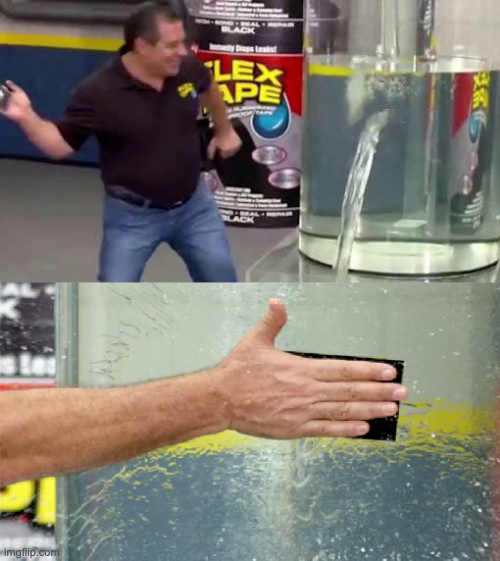
\includegraphics[width=0.5\textwidth]{images/flextape.png}
\end{center}

Applying some patches to the kernel like this should be rare and for emergencies, and ideally temporary until it's possible to have the next maintenance window. 

\end{frame}


\begin{frame}[fragile]
\frametitle{Patch Example}

\begin{lstlisting}[language=C]
#define pr_fmt(fmt) KBUILD_MODNAME ": " fmt

#include <linux/module.h>
#include <linux/kernel.h>
#include <linux/livepatch.h>

#include <linux/seq_file.h>
static int livepatch_cmdline_proc_show(struct seq_file *m, void *v)
{
	seq_printf(m, "%s\n", "this has been live patched");
	return 0;
}

static struct klp_func funcs[] = {
	{
		.old_name = "cmdline_proc_show",
		.new_func = livepatch_cmdline_proc_show,
	}, { }
};

static struct klp_object objs[] = {
	{
		/* name being NULL means vmlinux */
		.funcs = funcs,
	}, { }
};
\end{lstlisting}
\end{frame}


\begin{frame}[fragile]
\frametitle{Patch Example}
\begin{lstlisting}[language=C]
static struct klp_patch patch = {
	.mod = THIS_MODULE,
	.objs = objs,
};

static int livepatch_init(void)
{
	return klp_enable_patch(&patch);
}

static void livepatch_exit(void)
{
}

module_init(livepatch_init);
module_exit(livepatch_exit);
MODULE_DESCRIPTION("Kernel Live Patching Sample Module");
MODULE_LICENSE("GPL");
MODULE_INFO(livepatch, "Y");
\end{lstlisting}


\end{frame}


\begin{frame}
\frametitle{Shadow Variables}

The live patching implementation also allows something that the \texttt{kpatch} approach did not: changing kernel data structures!

  
 It's more like, what if we gave them companions.

\begin{center}
	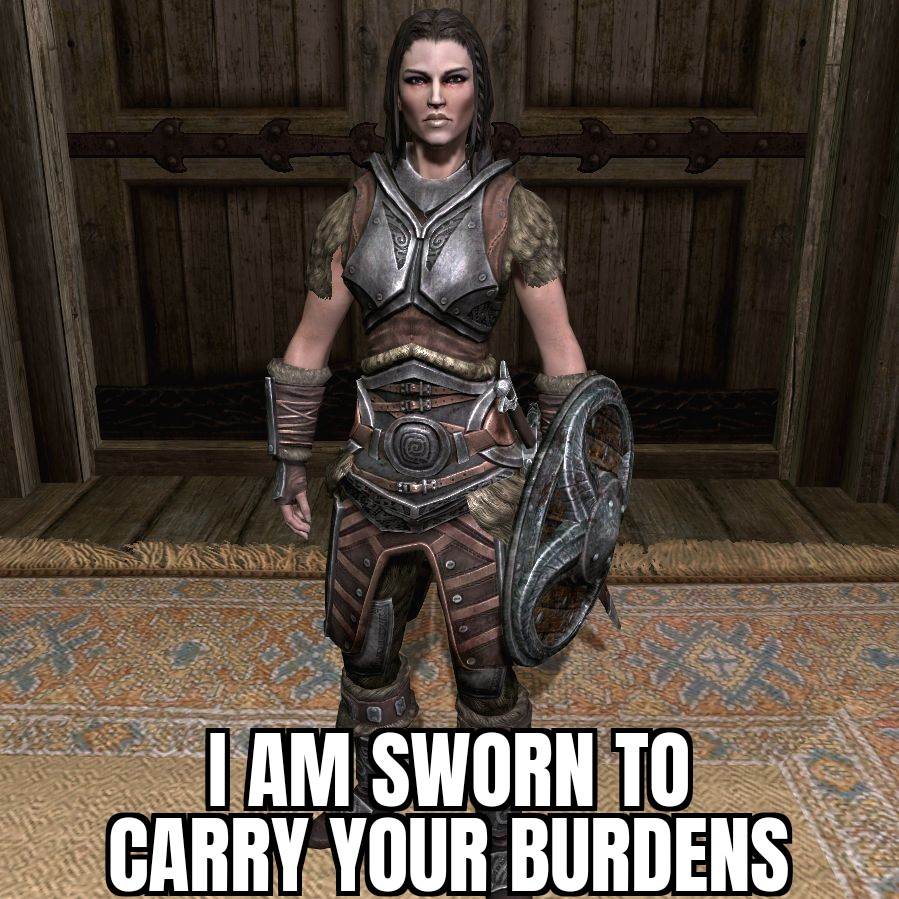
\includegraphics[width=0.4\textwidth]{images/lydia.jpg}
\end{center}


\end{frame}


\begin{frame}
\frametitle{Companion Objects}

Shadow variables allow attaching these extra companion objects to the existing data structures. 

So we're not really changing the originals, but we do get to put more things in the associated object. 

It's permitted to have multiple shadow variables attached to the same parent. 

\end{frame}


\begin{frame}
\frametitle{Companion Objects}
A shadow object has some identifier that tells us what the parent is; the kernel must also have a hash table to match.

We need to allocate the shadow variable structures and deallocate them explicitly.

This matters when the original is deallocated, but also when unloading the patch.

\end{frame}






\end{document}
